%\begin{figure}
%  \includegraphics[width=0.25\linewidth]{main_figures/test_figure.png}
%  \caption{A figure.}
%  \label{fig:test_fig}
%\end{figure}
%
%\newpage

In 2001, the first analyses of the draft human genome were published in sister papers in \textit{Nature} and \textit{Science}. The Human Genome Project had been budgeted US\$$3$~billion in 1990; by 2020 the cost of sequencing a human genome had dropped to US\$$1,000$, and a relative paucity of data had given way to abundance\citep{gibbs_human_2020}. Biobanks with data from tens or hundreds of thousands of individuals are becoming commonplace.

Every genome carries both the stories of its ancestors and the basic programming of its bearer's physiology. By identifying patterns across many genomes and their associated data, we can infer their histories and study distributions of biomedical traits. The complexities of human history and society, to say nothing of the complexities of biology itself, ensure that this is a non-trivial task.

With each genome spanning $3$~billion base pairs, any mathematical investigation is high-dimensional. This thesis explores applications of dimensionality reduction to population genetic data, focusing on uniform manifold approximation and projection (UMAP), a method of topological data analysis.

This thesis is organized into three chapters that have been published as stand-alone manuscripts. In \hyperref[chap:chapter1]{Chapter~1} we apply UMAP to human genetic data for the first time. We use genotype data from three biobanks, generating visualizations and observing patterns in relatedness, demographic histories, geographic distribution, phenotype distributions, and other phenomena. In \hyperref[chap:chapter2]{Chapter~2} we review the applications of UMAP in other human genetic datasets, such as different biobanks or other types of genetic data (e.g. structural variants). Finally, in \hyperref[chap:chapter3]{Chapter~3} we formalize a methodology to use UMAP in higher dimensions ($n \ge 3$) and extract clusters.

% high-level concepts?
% shape of data
% population structure
% complexity and interrelatedness

\section{Genetic diversity}

The human genome spans over $3$~billion nucleobase pairs organized across $23$ pairs of chromosomes---$22$ pairs of autosomes and one pair of sex chromosomes---with some DNA present in mitochondria (mtDNA). The human genome is diploid (i.e. paired) with one set of chromosomes coming from each parent via their gametes; these chromosomes are created through the process of meiotic recombination, in which the chromosomes of grandparents are aligned, cross over, and recombine. Along with mutation, recombination generates diversity. Approximately $99.9\%$ of DNA shared between humans is identical, with genetic variants (alleles) arising through mutations. Single nucleotide polymorphisms (SNPs) are relatively common variants, usually defined as having a frequency above $1\%$.

Variants that lie along the same chromosome and are not broken up through recombination are co-inherited and are linked. The block of allelic states along a DNA molecule is referred to as a haplotype, and when the same variants exist between two individuals, they are said to be identical by state (IBS). If the shared variant is inherited from a common ancestor without recombination, they are also said to be identical by descent (IBD); alleles that are IBS are typically IBD, with rare exceptions. Alleles that are physically closer are more likely to be inherited together, and those that appear together more often than expected at random are said to be in linkage disequilibrium (LD). Combining two haplotypes gives a diploid genotype, and assuming free recombination, the theoretical maximum number of possible unique haplotypes is $2^L$, where $L$ is the number of SNPs.

Recombination is not uniformly random. DNA that does not lie in the pseudoautosomal regions (PAR1 and PAR2) of the Y chromosome, as well as mtDNA, does not recombine\citep{jobling_human_2013}. Recombination rates also vary within chromosomes with certain regions known to be hotspots\citep{altemose_map_2017}. Germline mutations may result from copying errors during replication or from spontaneous errors from DNA’s instability or external factors like UV radiation. Whole genome sequencing pedigree-based studies estimate the overall mutation rate at about $10^{-8}$ per base pair per generation, though this rate may vary depending on the mechanistic source of the mutation\citep{segurel_determinants_2014}.

\subsection{Population structure}

% what does structure *look* like?

In aggregate, patterns will form in the distributions of alleles; these patterns are known as population structure. Though genetic diversity is random in principle, the distributions of variants are shaped by environments and events. Phenomena like migrations, population bottlenecks, and non-random mating contribute to the distribution of alleles.

Why is genetic variation not fully random? How do we measure it? What are the processes that we know of? What are some historical examples?

\subsection{Measures of population structure}

\subsubsection{Hardy-Weinberg Equilibrium}

\subsubsection{Fixation index}

\subsection{Ancestry and admixture}

\section{Exploratory data analysis}

Traditional statistical analyses of biological data follow the recommendations of R.A. Fisher in the 1930s\citep{holmes_modern_2019}. They have a linear structure: beginning with a biological question, an investigator forms a hypothesis and an associated null ($H_0$), designs an experiment, collects data, tests $H_0$ with a p-value, and formulates a conclusion. Beginning in the 1970s, statistician John W. Tukey proposed the alternative framework of exploratory data analysis (EDA)\citep{tukey_1977,hoaglin_john_2003}. This approach is iterative and instead begins with the data: we visualize it, understand it, and use it to inform what sort of analysis to use in an accompanying confirmatory data analysis. The two contrasting approaches are schematized in Figure~\ref{fig:paradigms}.

\begin{figure}[h!]
\centering
\begin{subfigure}{0.3\textwidth}
    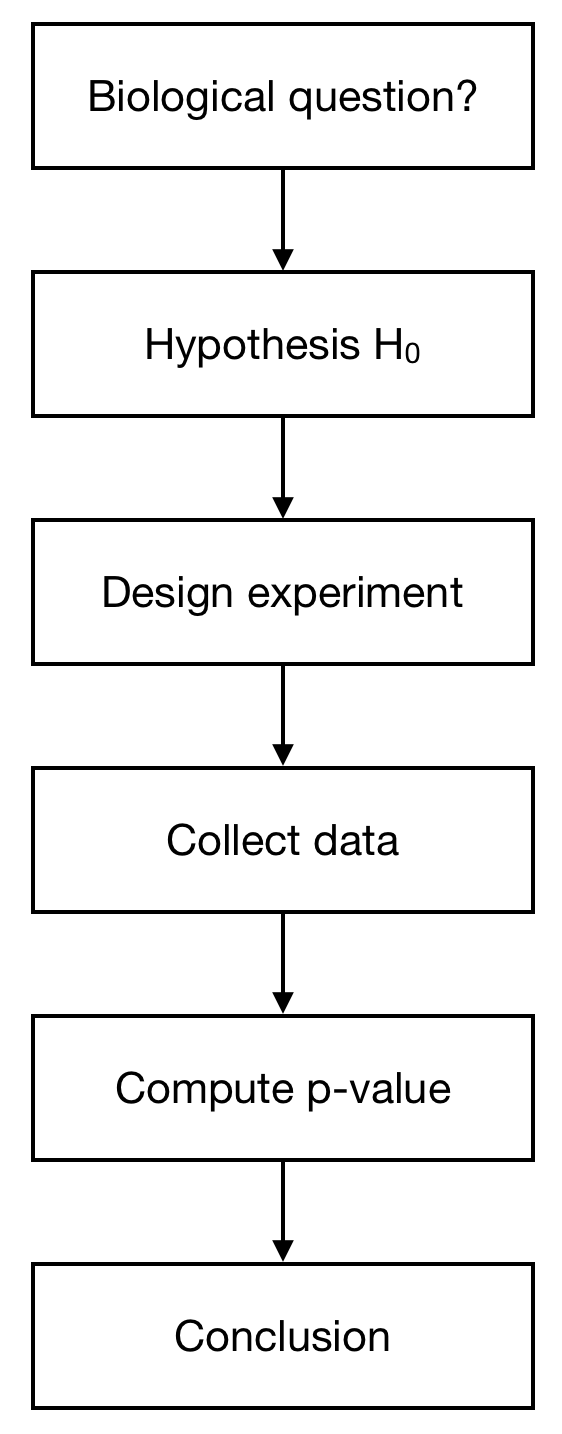
\includegraphics[height=0.5\textheight]{main_figures/intro/fisher_paradigm.png}
    \caption{Fisher's paradigm.}
    \label{fig:fisher}
\end{subfigure}
\hfill
\begin{subfigure}{0.65\textwidth}
    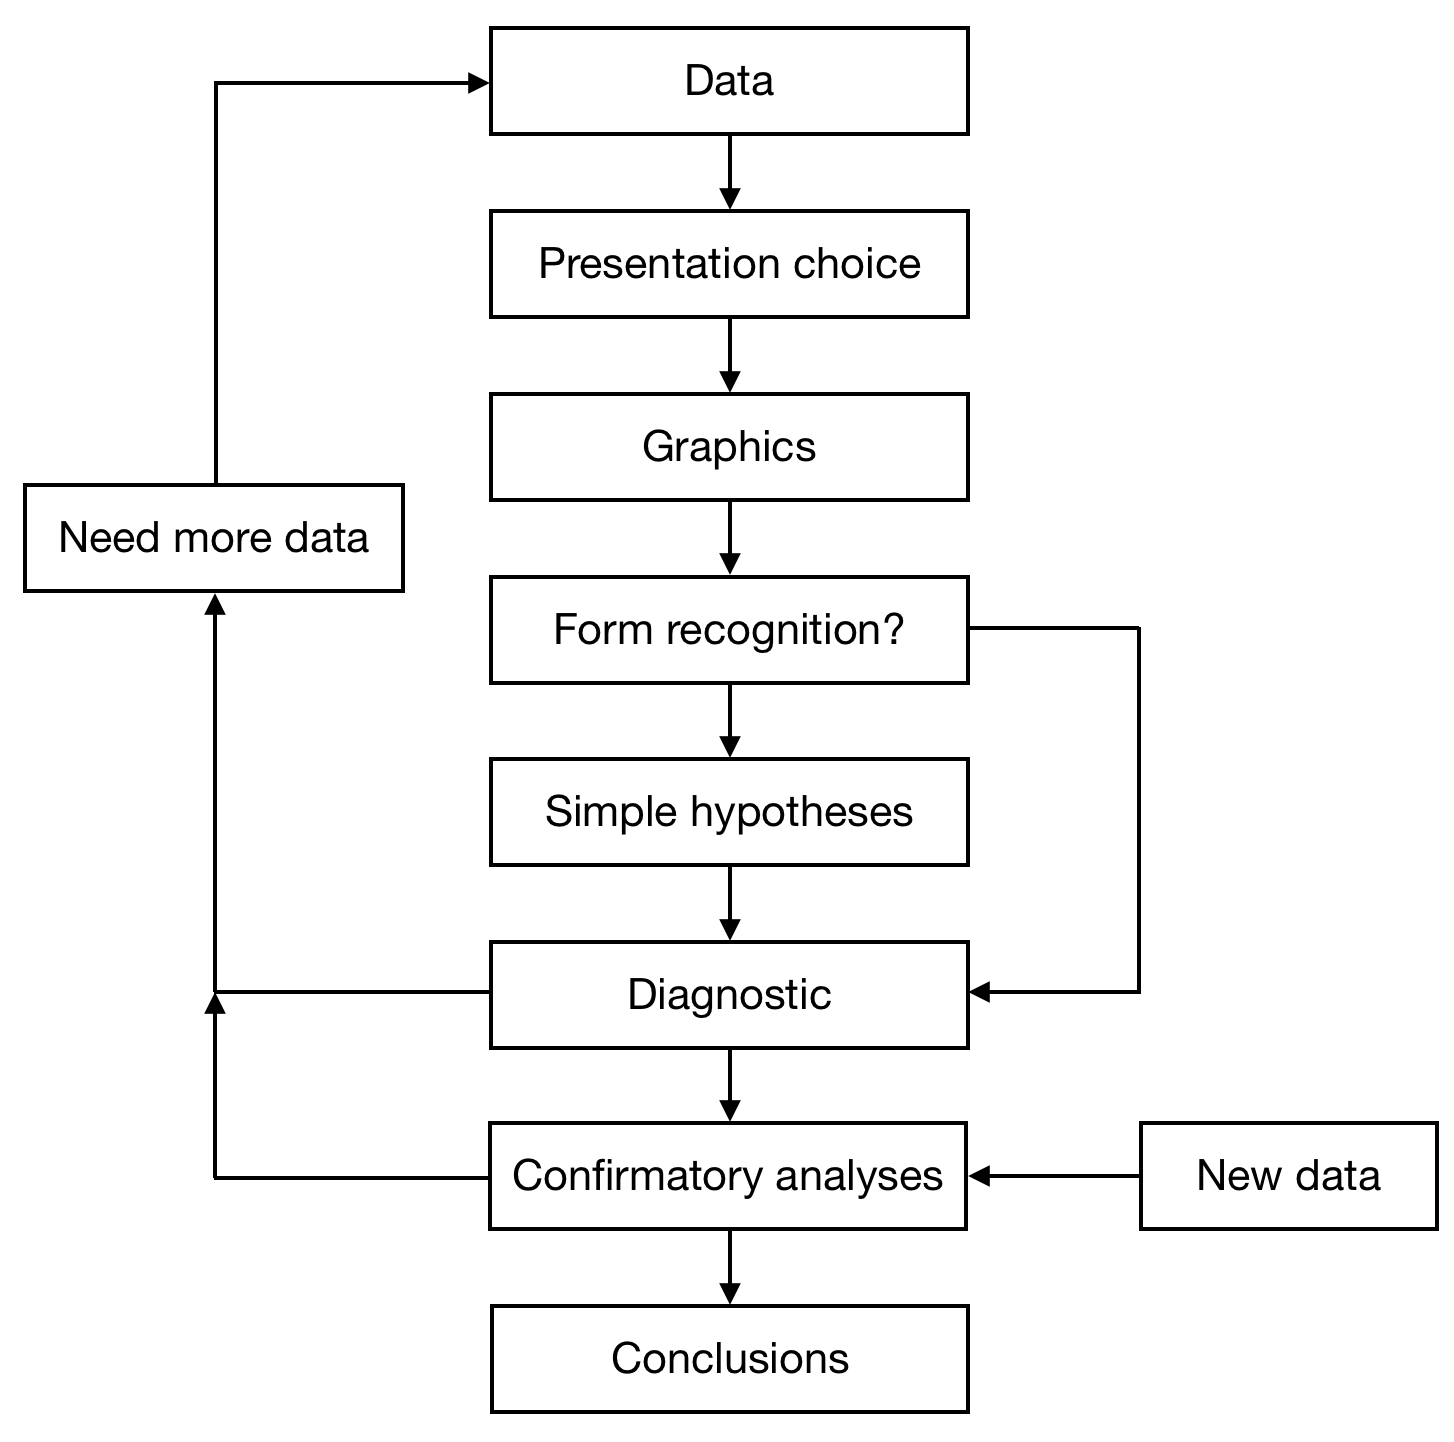
\includegraphics[height=0.5\textheight]{main_figures/intro/tukey_paradigm.png}
    \caption{Tukey's paradigm.}
    \label{fig:tukey}
\end{subfigure}
\caption{\textbf{Contrasting Fisher's paradigm with Tukey's paradigm in biology.} Fisher's paradigm (left) takes a sequential approach to data analysis, beginning with a well-defined question and strong assumptions. Tukey's paradigm (right) is iterative, beginning with the data, emphasizing exploratory analysis through visualization, and complemented by confirmatory analyses that are robust and do not rely on complex assumptions\citep{holmes_modern_2019}.}
\label{fig:paradigms}
\end{figure}

Writing in 1980, Tukey emphasized that science neither begins with a tidy question nor ends with a tidy answer\citep{tukey_we_1980}. This is especially true in modern biology. Statistical questions from the 1930s typically had a few parameters $p$ with a manageable sample size $N$ (where $N > p$), and the people posing questions were involved in data collection. Today we sit at the opposite extreme; it is not unusual for data to have $p >> N$ with the two values differing by orders of magnitude. When studying a biobank, we may have several thousand individuals and several hundred thousand genetic markers. Generally, the people investigating data have not collected it. These factors make Tukey's paradigm much better suited to our analytical needs\citep{holmes_modern_2019}. 

\subsection{Dimensionality reduction}

In Figure~\ref{fig:tukey}, the iterative process includes presentation choices, graphics, and form recognition. This provokes a natural question: what approaches ought we use here? With genomic data comes the ``curse of dimensionality'': though we have many dimensions to our data, the signal is sparse and many methods are computationally intractable. This motivates dimensionality reduction---we wish to reduce our data to a relatively low number of dimensions, ideally preserving important characteristics of the data. Given a satisfactory representation of the data set, we can visualize it.

\subsubsection{Principal component analysis}
Principal components analysis (PCA) is a non-parametric linear transformation that projects data onto a series of orthogonal axes based on a linear combination of the original data. The axes are generated and ordered according to their eigenvalues, and the ratio of each axis' corresponding eigenvalue to the sum of all eigenvalues represents the variance explained by that axis. PCA fits an ellipsoid around the data in high dimensions and the axes of that ellipsoid are the principal components. By only selecting the largest axes---corresponding to the most explained variance --- we can reduce the dimensionality of our data while preserving significant explanatory value. We can also interpret our dimensionally reduced data in terms of how much of the overall variance it explains. Principal components are calculated through eigendecomposition of the covariance matrix; a derivation for genotype data is given in \hyperref[appendix:AppendixA]{Appendix~A}. A detailed examination of PCA in the context of population genetics can be found in \citep{mcvean_genealogical_2009}. 

PCA has seen wide application in population genetics. The top PCs often reflect isolation-by-distance and are used for visualization (e.g. within Europe\citep{novembre2008europe}). However, using them for visualization requires selecting which components to examine and is limited to $2$ or $3$ dimensions; if there is signal beyond the first few PCs, it may go unnoticed. We expand on this in \hyperref[chap:chapter1]{Chapter~1}.

They are also used to correct for population structure in genome-wide association studies (GWAS) by their inclusion as covariates in models\cite{price_principal_2006}. There are varying rules-of-thumb on how many PCs to include in a model, such as using the top $10$, looking for an ``elbow'' in the scree plot, or testing for eigenvalue significance in the Wishart distribution; however, these are merely conventions. We explore the impact of PC adjustment for phenotypes in biobanks in \hyperref[chap:chapter3]{Chapter~3}. 

\subsection{Topological data analysis}

% Note to self: Rewrite this in terms of popgen challenges
% can maybe get philosophical here
We are often interested in learning about our data in to understand its large-scale structure, e.g., identifying different cell types or related individuals. Though we have some definitions of distances, we are interested in notions of \textit{similarity} or \textit{nearness}. Topology provides the mathematical machinery for ideas rooted in qualitative geometry\citep{carlsson_topology_2009}. Topological data analysis (TDA) is a set of statistical methods that uses ideas of shape and connectivity to study data\citep{wasserman_topological_2018}. We will focus on applications of manifold learning, non-linear dimensionality reduction, and density clustering.

TDA assumes that we observe a sample $X_1, \dots, X_n \sim P$ with $P$ supported on some set $\supp(P) = \mathcal{X} \subseteq \mathbb{R}^d$. 
In the simplest case of manifold learning, we suppose that $P$ is actually supported on some set $S$ with dimension $r$, where $r < d$ and $S$ is a smooth and compact manifold, and we may estimate $S$. PCA is a special case of linear manifold learning where data are assumed to lie on or near an affine subspace\citep{wasserman_topological_2018}. In cases where there is local nonlinear structure (such as clustering), nonlinear methods of manifold learning are more useful\cite{izenman_introduction_2012}.

In population genetics, we observe samples from, e.g., the distributions of genotypes.

\subsection{\texorpdfstring{$\mathbf{t}$}{f}-distributed stochastic neighbour embedding}
% the {f} here doesn't do anything, but we need a text character for compilation

$t$-distributed stochastic neighbour embedding ($t$-SNE) is a method of manifold learning used for visualization that was developed in 2008\citep{maaten_visualizing_2008}. By then, several methods existed to approximate the local structure of manifolds, but they suffered from the ``crowding problem''---in an attempt to preserve local distances between points, many of them are crunched together, eliminating the gaps between clusters. $t$-SNE addressed this by introducing a repulsion force between points, modelling pairwise distances between points $i$ and $j$ as a $t$-distributed random variable with $1$ degree of freedom (equivalent to a Cauchy distribution). The distances are modelled as probabilities:

$$q_{ij} = \frac{(1 + ||y_{i} - y_{j}||^{2})^{-1}}{\sum_{k \neq l}(1 + ||y_{k} - y_{l}||^{2})^{-1}}$$

This choice was largely ad-hoc and was later found to work because it optimized structure at the local scale (i.e. within clusters) as well as causing points to repel each other (i.e. causing clusters to separate)\citep{carreira-perpinan_elastic_2010}. This repulsion allowed $t$-SNE and related methods to preserve topology\citep{wasserman_topological_2018}. Because $t$-SNE can only reduce data to $2$ or $3$ dimensions, it was not recommended as a general purpose dimensionality reduction algorithm\citep{maaten_visualizing_2008}. It saw considerable use in visualization in single-cell genomics\citep{kobak_art_2019}, but its application in population genetics was limited (e.g. \citep{li_application_2017}). We provide details on $t$-SNE's performance in population genetics in \hyperref[chap:chapter1]{Chapter~1}.

\subsection{Uniform manifold approximation and projection}

Uniform manifold approximation and projection (UMAP) is a general purpose dimensionality reduction method rooted in algebraic topology and Riemannian geometry that was introduced in 2018\citep{mcinnes_umap_2020}. Unlike the more heuristic approach of $t$-SNE, the motivation behind UMAP is to represent the high-dimensional topology of data in low dimensional space. We will briefly outline the intuition underlying UMAP; details on the topology and theoretical justifications are available in \citep{mcinnes_umap_2020}, with a more applied explanation available in online documentation\citep{mcinnes_umapdoc_2018}.

We assume our data $X = \{X_{1}, \dots, X_{n}\}$ lay on some manifold and are uniformly distributed. For this assumption to hold, each point $X_{i}$ has its own custom distance, defined as the normalized distance to its $k\textsuperscript{th}$ nearest neighbour; thus, each $X_{i}$ has its own metric space, and is the centre of a unit ball that extends to the $k\textsuperscript{th}$ nearest neighbour. If we represent this as a graph, each $X_i$ is a point with edges to its $k$ neighbours, where the distances represent the edge weights. If we represent this as a simplicial complex, a point is a $0$-simplex and an edge is a $1$-simplex; according to theory, this simplicial complex forms an open cover of the underlying topological space. As the edge weights are between $0$ and $1$, we may also interpret the values as the belongingness to an open cover rather than a binary ``yes'' or ``no'' value---a fuzzy topological cover. To harmonize the respective edge weights $a, b$ from points $X_{a}$ to $X_{b}$ (since each point has its own local metric), UMAP defines the combined weight as $a + b - a \times b$, interpreted as the probability that an edge weight between $X_{a}$ and $X_{b}$ exists. The final high-dimensional product is a fuzzy simplicial complex, which can be represented as a weighted graph, and is a fuzzy topological representation of the data.

For the low-dimensional representation, we carry out the same process of building a fuzzy topological representation. However, rather than using a locally-varying metric, we assume that our data will lay on a low-dimensional Euclidean space, and we specify a minimum distance we wish to have between our points in this space. The algorithm then minimizes the cross-entropy function between the high- and low-dimensional representations. If $E$ is the set of all possible $1$-simplices, $w_{h}(e)$ is the weight of edge $e$ in the high-dimensional space and $w_{l}(e)$ the low-dimensional space, we minimize:

$$ \sum_{e \in E} w_{h}(e) \log{\left(\frac{w_{h}(e)}{w_{l}(e)}\right)} + (1 - w_{h}(e)) \log{\left(\frac{1 - w_{h}(e)}{1 - w_{l}(e)}\right)} $$

Though the machinery seems roundabout in its derivation, it allows for reduction of data to an arbitrary number of dimensions and for topological interpretations. The value of $k$ defines the scale of the topology we wish to approximate, with lower values being more local and finer-scale and higher values approximating broader manifold structure. Each chapter of this thesis discusses the uses and parametrizations of UMAP in population genetics: briefly, lower values of $k$ approximate closer relationships, e.g., at a structure as fine-scale as families; higher values of minimum distance facilitate visualization, while lower values facilitate algorithmic cluster detection.

UMAP is the core method of this thesis. In \hyperref[chap:chapter1]{Chapter~1}, we use UMAP in population genetics for the first time, exploring its potential applications thoroughly and compare it to PCA and t-SNE. Having been quickly adopted after our publication, in \hyperref[chap:chapter2]{Chapter~2}, we review its uses in the field and discuss different data inputs and parametrizations. In \hyperref[chap:chapter3]{Chapter~3}, we introduce the use of UMAP for topological stratification of complex biobank data by using it to pre-process data for clustering rather than simply visualization.

``Is it possible to derive low dimensional embedding methods that explicitly preserve topological features of the data? This is an interesting open question.''\citep{wasserman_topological_2018}

\subsection{Clustering}

It can be useful to model populations as $K$ discrete demes, e.g. when modelling admixture, studying population splits and merges, or testing the transferability of GWAS and PGS. Clustering is a natural approach to this problem. Broadly, clustering is a class of methods that puts similar data points into the same cluster while keeping dissimilar data points in different clusters\citep{ben-david_clustering_2018}. A variety of clustering methods have been used in population genetics. These methods often require specifying $K$; though multiple methods have been proposed to estimate $K$ (e.g. \citep{evanno_detecting_2005,verity_estimating_2016}), though $K$ may be useful, it does not have a ``correct'' value as genetic data does not fall into natural discrete groups\citep{lawson_tutorial_2018}.

Model-based clustering assumes that observations are randomly drawn from some parametric model. The first such method used in population genetics was STRUCTURE, in 2000, which assumed that each cluster was defined by some allele frequency; having observed the genotypes $X$, it infers the populations of origin $Z$ and allele frequencies $P$ through Bayesian modelling of $Pr(Z, P|X)$\citep{pritchard_inference_2000}. Each genome is then modelled as a mixture of some $K$ source populations---often presented in literature as a stacked bar graph where each individual is one bar with split ancestry proportions---and termed ``global ancestry estimation''\citep{alexander_fast_2009}. The idea has since evolved into many other methods (e.g. ADMIXTURE\citep{alexander_fast_2009}, FRAPPE\citep{tang_estimation_2005}, sparse non-negative matrix factorization\citep{frichot_fast_2014}, archetypal analysis\citep{gimbernat-mayol_archetypal_2022}) and is an active area of research to handle more complex model assumptions and larger data sets.

One of the most common distance-based algorithms is $K$-means clustering. Developed in the 1970s, it works by dividing $M$ points in $N$ dimensions into $K$ groups by minimizing the within-cluster sum of squares\citep{hartigan_algorithm_1979}. $K$-means clustering has been used to define populations by, e.g., using the coordinates of individuals in PCA space and comparing to some known reference population within a cluster. $K$-means implicitly assumes that data points form a Gaussian cloud around some centroid\citep{mcinnes_accelerated_2017}. However, genetic data do not naturally present as clouds about some centroid---many individuals, particularly from admixed populations or uncommon genetic ancestries, will never be placed into a population, especially if there is no reference population\citep{ding_polygenic_2023}.

Density clustering 


 
\subsection{Density clustering}

\subsection{Visualization}

% some principles of visualization?

% unsupervised learning?

% clustering in popgen?

%\subsection{HDBSCAN(\texorpdfstring{$\hat{\epsilon}$}{f})}
% the {f} here doesn't do anything, but we need a text character for compilation

\citep{mcinnes_accelerated_2017}

\section{Data}

This research makes use of data from four biobanks. We focus on genotype data coded as the number of non-reference alleles. Given a set of $L$ SNPs for $N$ individuals, the genotype matrix $G$ is:

%$$
%G = \begin{bmatrix} 
%    g_{11} & g_{12} & \dots g_{1L} \\
%    \vdots & \ddots & \\
%    g_{N1} &        & g_{NL} 
%    \end{bmatrix}
%    
%\text{ where } g_{ij}\text{ is the number of non-reference alleles for individual } i \text{ at locus } j.
%$$

\subsection{The 1000 Genomes Project}

The 1000 Genomes Project (1KGP) is a publicly available data set of genetic data sampled from many populations from around the world\citep{global_2015}. We used $3,450$ genotypes from the Affy 6.0 platform sampled from $26$  populations. The populations sizes are roughly similar, with between $104$ to $183$ in each group.

\subsection{CARTaGENE}

CARTaGENE (CaG) is a cohort of residents of Qu\'{e}bec with genotype data for $29,337$ participants, who were recruited using registration data from the R\'{e}gie de l’assurance maladie du Qu\'{e}bec (RAMQ), the provincial health authority\citep{awadalla_cohort_2013}. In addition to genetic data, it contains questionnaire health data and demographic information such as country of birth and ethnicity.

\subsection{Health and Retirement Study}

The Health and Retirement Study (HRS) is a cohort of retired American individuals\citep{juster_overview_1995}. We used genotype data from 12,454 individuals from the Health and Retirement Study (HRS), genotyped on the Illumina Human Omni 2.5M platform. The database contains basic demographic data such as age, US Census Bureau region of birth, and race.

\subsection{UK biobank}

The UK biobank (UKB) is a cohort of individuals living in the United Kingdom who were recruited by inviting those registered with the National Health Service (NHS)\citep{sudlow_uk_2015}. It contains the genotypes from $488,377$ participants as well as detailed health data, phenotypic measures, geographic coordinates, and sociodemographic information such as ethnic background.

%\section{Methods}

%\subsection{PCA}

%\subsection{UMAP}

%\subsection{Genomic tools}